\begin{figure*}[t]
  \centering
    \noindent
    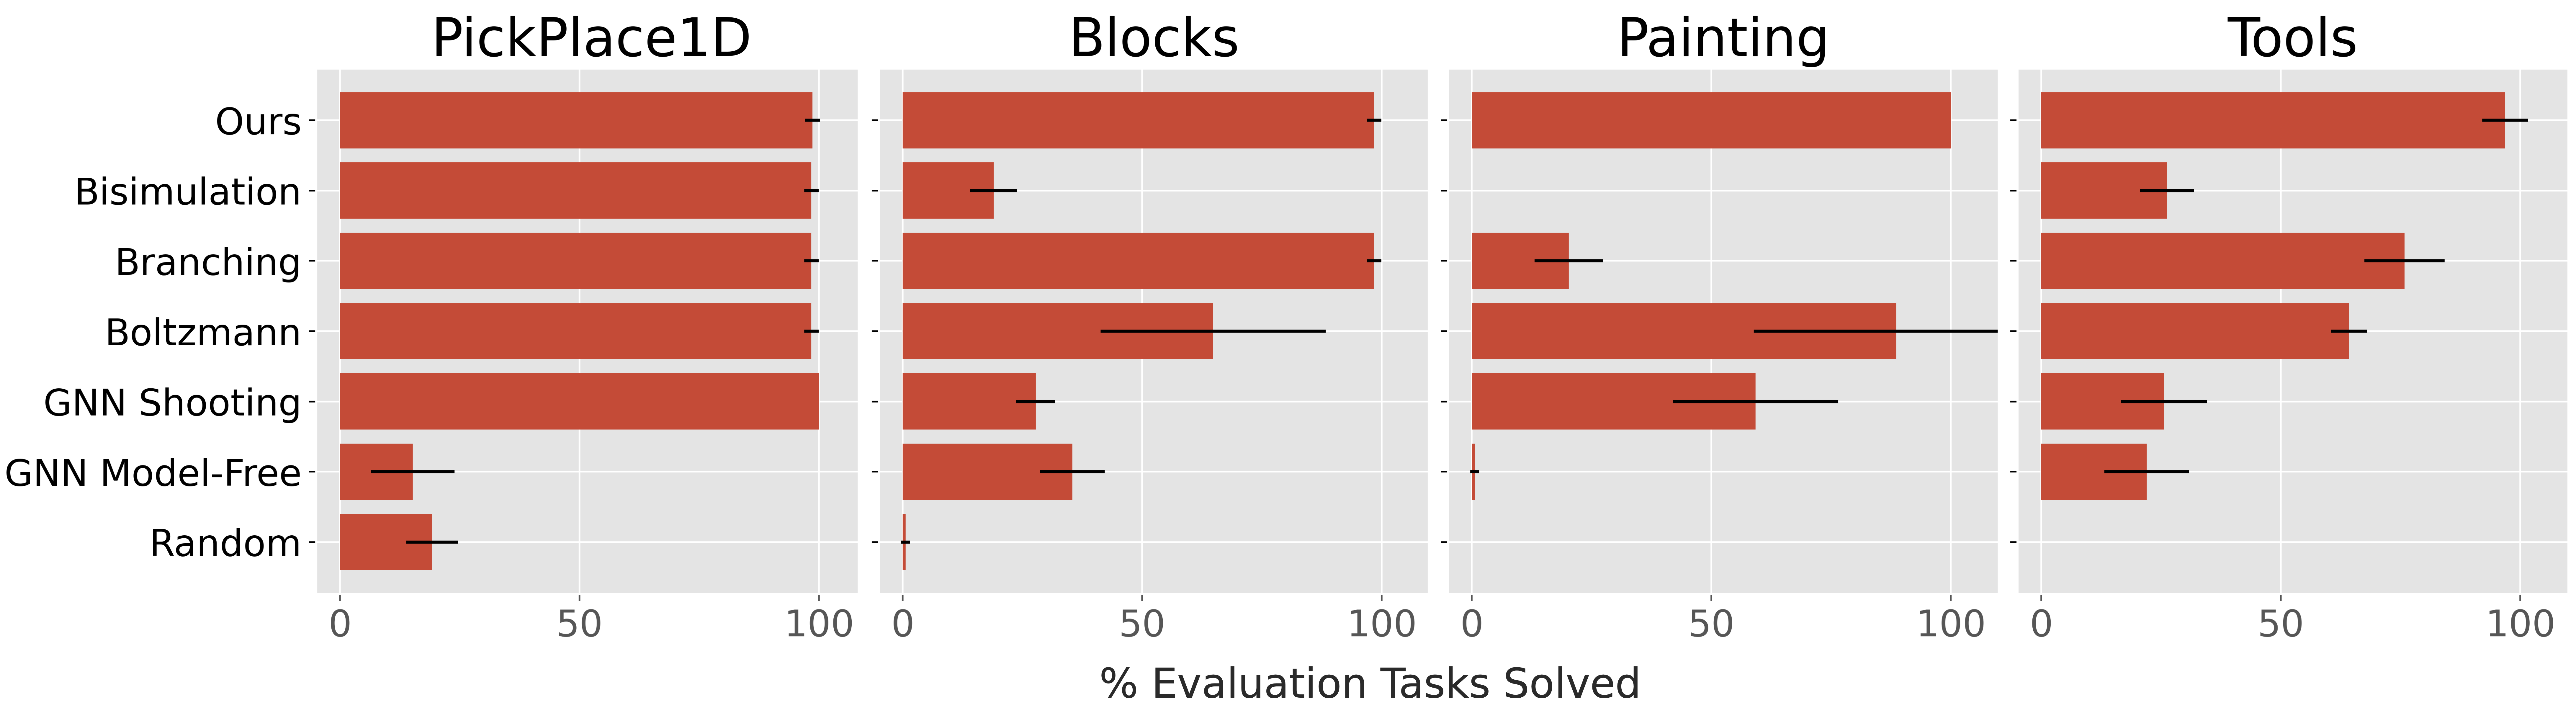
\includegraphics[width=\textwidth]{figures/barplots.png}
    \caption{\small{\textbf{Ours versus baselines.} Percentage of 50 evaluation tasks solved under a 10-second timeout, for all four environments. All results are averaged over 10 seeds. Black bars denote standard deviations.
    Learning times and additional metrics are reported in \appref{app:results}.}}
  \label{fig:barplots}
\end{figure*}

\begin{table*}
	\centering
	\resizebox{0.85\textwidth}{!}{%
    \begin{tabular}{| l | p{0.75cm} | p{0.75cm} | p{0.75cm} || p{0.75cm} | p{0.75cm} | p{0.75cm} || p{0.75cm} | p{0.75cm} | p{0.75cm} || p{0.75cm} | p{0.75cm} | p{0.75cm} | }
	\hline
	\multicolumn{1}{|c|}{} &\multicolumn{3}{c||}{\bf{Ours}} &
	\multicolumn{3}{c||}{\bf{Manual}} &
	\multicolumn{3}{c||}{\bf{Down Eval}} &
	\multicolumn{3}{c|}{\bf{No Invent}} \\
	\hline
	\bf{Environment} &
	{Succ} & {Node} & {Time}&
	{Succ} & {Node} & {Time}&
	{Succ} & {Node} & {Time}&
	{Succ} & {Node} & {Time}\\
	\hline
	PickPlace1D & 98.6 & 4.8 & 0.006 & 98.4 & 6.5 & 0.045 & 98.6 & 4.8 & 0.008 & 39.6 & 14.1 & 1.369 \\
	Blocks & 98.4 & 2949 & 0.296 & 98.6 & 2941 & 0.251 & 98.2 & 2949 & 0.318 & 3.2 & 427.7 & 1.235 \\
	Painting & 100.0 & 501.8 & 0.470 & 99.6 & 2608 & 0.464 & 98.8 & 489.0 & 0.208 & 0.0 & \;\;\;-- & \;\;\;-- \\
	Tools & 96.8 & 1897 & 0.457 & 100.0 & 4771 & 0.491 & 42.8 & 152.5 & 0.060 & 0.0 & \;\;\;-- & \;\;\;-- \\\hline
	\end{tabular}}
    
	\caption{\small{\textbf{Ours versus Manual and ablations.} Percentage of 50 evaluation tasks solved under a 10-second timeout (Succ), number of nodes created during \textsc{GenAbstractPlan} (Node), and wall-clock planning time in seconds (Time). All results are averaged over 10 seeds. The Node and Time columns average over \emph{solved tasks only}. Standard deviations are provided in \appref{app:results}.}}
	\label{tab:ablations}
\end{table*}

% Our experiments investigate the extent to which abstractions learned with our approach enable efficient planning.

Our experiments are designed to answer the following questions:
\textbf{(Q1)} To what extent do our learned abstractions help both the effectiveness and the efficiency of planning, and how do they compare to abstractions learned using other objective functions?
\textbf{(Q2)} How do our learned state abstractions compare in performance to manually designed state abstractions?
\textbf{(Q3)} How data-efficient is learning, with respect to the number of demonstrations?
\textbf{(Q4)} Do our abstractions vary as we change the planner configuration, and if so, how?

\subsubsection{Experimental Setup}
We evaluate 10 methods across four robotic planning environments.
All results are averaged over 10 random seeds.
For each seed, we sample a set of 50 \emph{evaluation tasks} that involve more objects and harder goals than were seen at training.
Demonstrations are collected by bilevel planning with manually defined abstractions (see Manual method below).
%Our key measures of \emph{effective and efficient planning} are (1) success rate  and (2) wall-clock time.
Planning is always limited to a 10-second timeout.
See \appref{app:additional-experimental-details} for additional details.

\subsubsection{Environments} We now briefly describe the environments, with further details in \appref{app:details}. The first three environments were established in prior work by ~\citet{silver2021learning}, but in that work, all predicates were manually defined; we use the same predicates in the Manual baseline.
\begin{tightlist}
\item \textbf{PickPlace1D.} A robot must pick blocks and place them onto target regions along a table surface. All pick and place poses are in a 1D line. 
Evaluation tasks require 1-4 actions to solve.
\item \textbf{Blocks.} A robot in 3D must interact with blocks on a table to assemble them into towers. This is a robotic version of the classic blocks world domain.
Evaluation tasks require 2-20 actions to solve.
\item \textbf{Painting.} A robot in 3D must pick, wash, dry, paint, and place widgets into either a box or a shelf.
Evaluation tasks require 11-25 actions to solve.
\item \textbf{Tools.} A robot operating on a 2D table surface must assemble contraptions with screws, nails, and bolts, using a provided set of screwdrivers, hammers, and wrenches respectively. This environment has physical constraints that cannot be modeled by our predicate grammar.
Evaluation tasks require 7-20 actions to solve.
\end{tightlist}

\subsubsection{Methods} We evaluate our method, six baselines, a manually designed state abstraction, and two ablations.
Note that the Bisimulation, Branching, Boltzmann, and Manual baselines differ from Ours only in predicate learning.
\begin{tightlist}
\item \textbf{Ours.} Our main approach.
\item \textbf{Bisimulation.} A baseline that learns abstractions by approximately optimizing the \emph{bisimulation criteria}~\cite{givan2003equivalence}, as in prior work~\cite{curtis2021discovering}. Specifically, this baseline learns abstractions that minimize the number of transitions in the demonstrations where the abstract transition model $F$ is applicable but makes a misprediction about the next abstract state. Note that because goal predicates are given, goal distinguishability is satisfied under any abstraction.
\item \textbf{Branching.} A baseline that learns abstractions by optimizing the \emph{branching factor} of planning. Specifically, this baseline learns predicates that minimize the number of applicable operators over demonstration states.
\item \textbf{Boltzmann.} A baseline that assumes the demonstrator is acting \emph{noisily rationally} under (unknown) optimal abstractions~\cite{baker2009action}. For any candidate abstraction, we compute the likelihood of the demonstration under a Boltzmann policy using the planning heuristic as a surrogate for the true cost-to-go.
\item \textbf{GNN Shooting.} A baseline that trains a graph neural network~\cite{battaglia2018relational} policy. This GNN takes in the current state $x$, abstract state $s$, and goal $g$. It outputs an action $a$, via a one-hot vector over $\C$ corresponding to which controller to execute, one-hot vectors over all objects at each discrete argument position, and a vector of continuous arguments. We train the GNN using behavior cloning on the data $\D$. At evaluation time, we sample trajectories by treating the outputted continuous arguments as the mean of a Gaussian with fixed variance. We use the transition model $f$ to check if the goal is achieved, and repeat until the planning timeout is reached.
\item \textbf{GNN Model-Free.} A baseline that uses the same GNN, but directly executes the policy instead of shooting.
\item \textbf{Random.} A baseline that simply executes a random controller with random arguments on each step. No learning.
\item \textbf{Manual.} An oracle approach that plans with manually designed predicates for each environment.
\item \textbf{Down Eval.} An ablation of Ours that uses $n_{\text{abstract}} = 1$ during evaluation only, in \textsc{Plan} (\algref{alg:plan}).
\item \textbf{No Invent.} An ablation of Ours that uses $\Psi = \Psi_G$, i.e., only goal predicates are used for the state abstraction.
\end{tightlist}




\subsubsection{Results and Discussion}


We provide real examples of learned predicates and operators for all environments in \appref{app:results}.
\figref{fig:barplots} shows that our method solves many more held-out tasks within the timeout than the baselines.
A major reason for this performance gap is that our surrogate objective $J_{\text{surr}}$ explicitly approximates the efficiency of planning.
The lackluster performance of the bisimulation baseline is especially notable because of its prevalence in the literature~\cite{pasula2007learning, jetchev2013learning,bonet2019learning,curtis2021discovering}.
We examined its failure modes more closely and found that it consistently selects good predicates, but not \emph{enough} of them.
This is because requiring the operators to be a perfect predictive model in the abstract spaces is often not enough to ensure good planning performance. For example, in the Blocks environment, the goal predicates together with the predicate \texttt{Holding(?block)} are enough to satisfy bisimulation on our data, while other predicates like \texttt{Clear(?block)} and \texttt{HandEmpty()} are useful from a planning perspective.
Examining the GNN baselines, we see that while shooting is beneficial versus using the GNN model-free, the performance is generally far worse than Ours.
Additional experimentation we conducted suggests that the GNN gets better with around an order of magnitude more data.

\begin{wrapfigure}[10]{r}{0.29\textwidth}
\vspace{-1.5em}
\hspace{-1em}
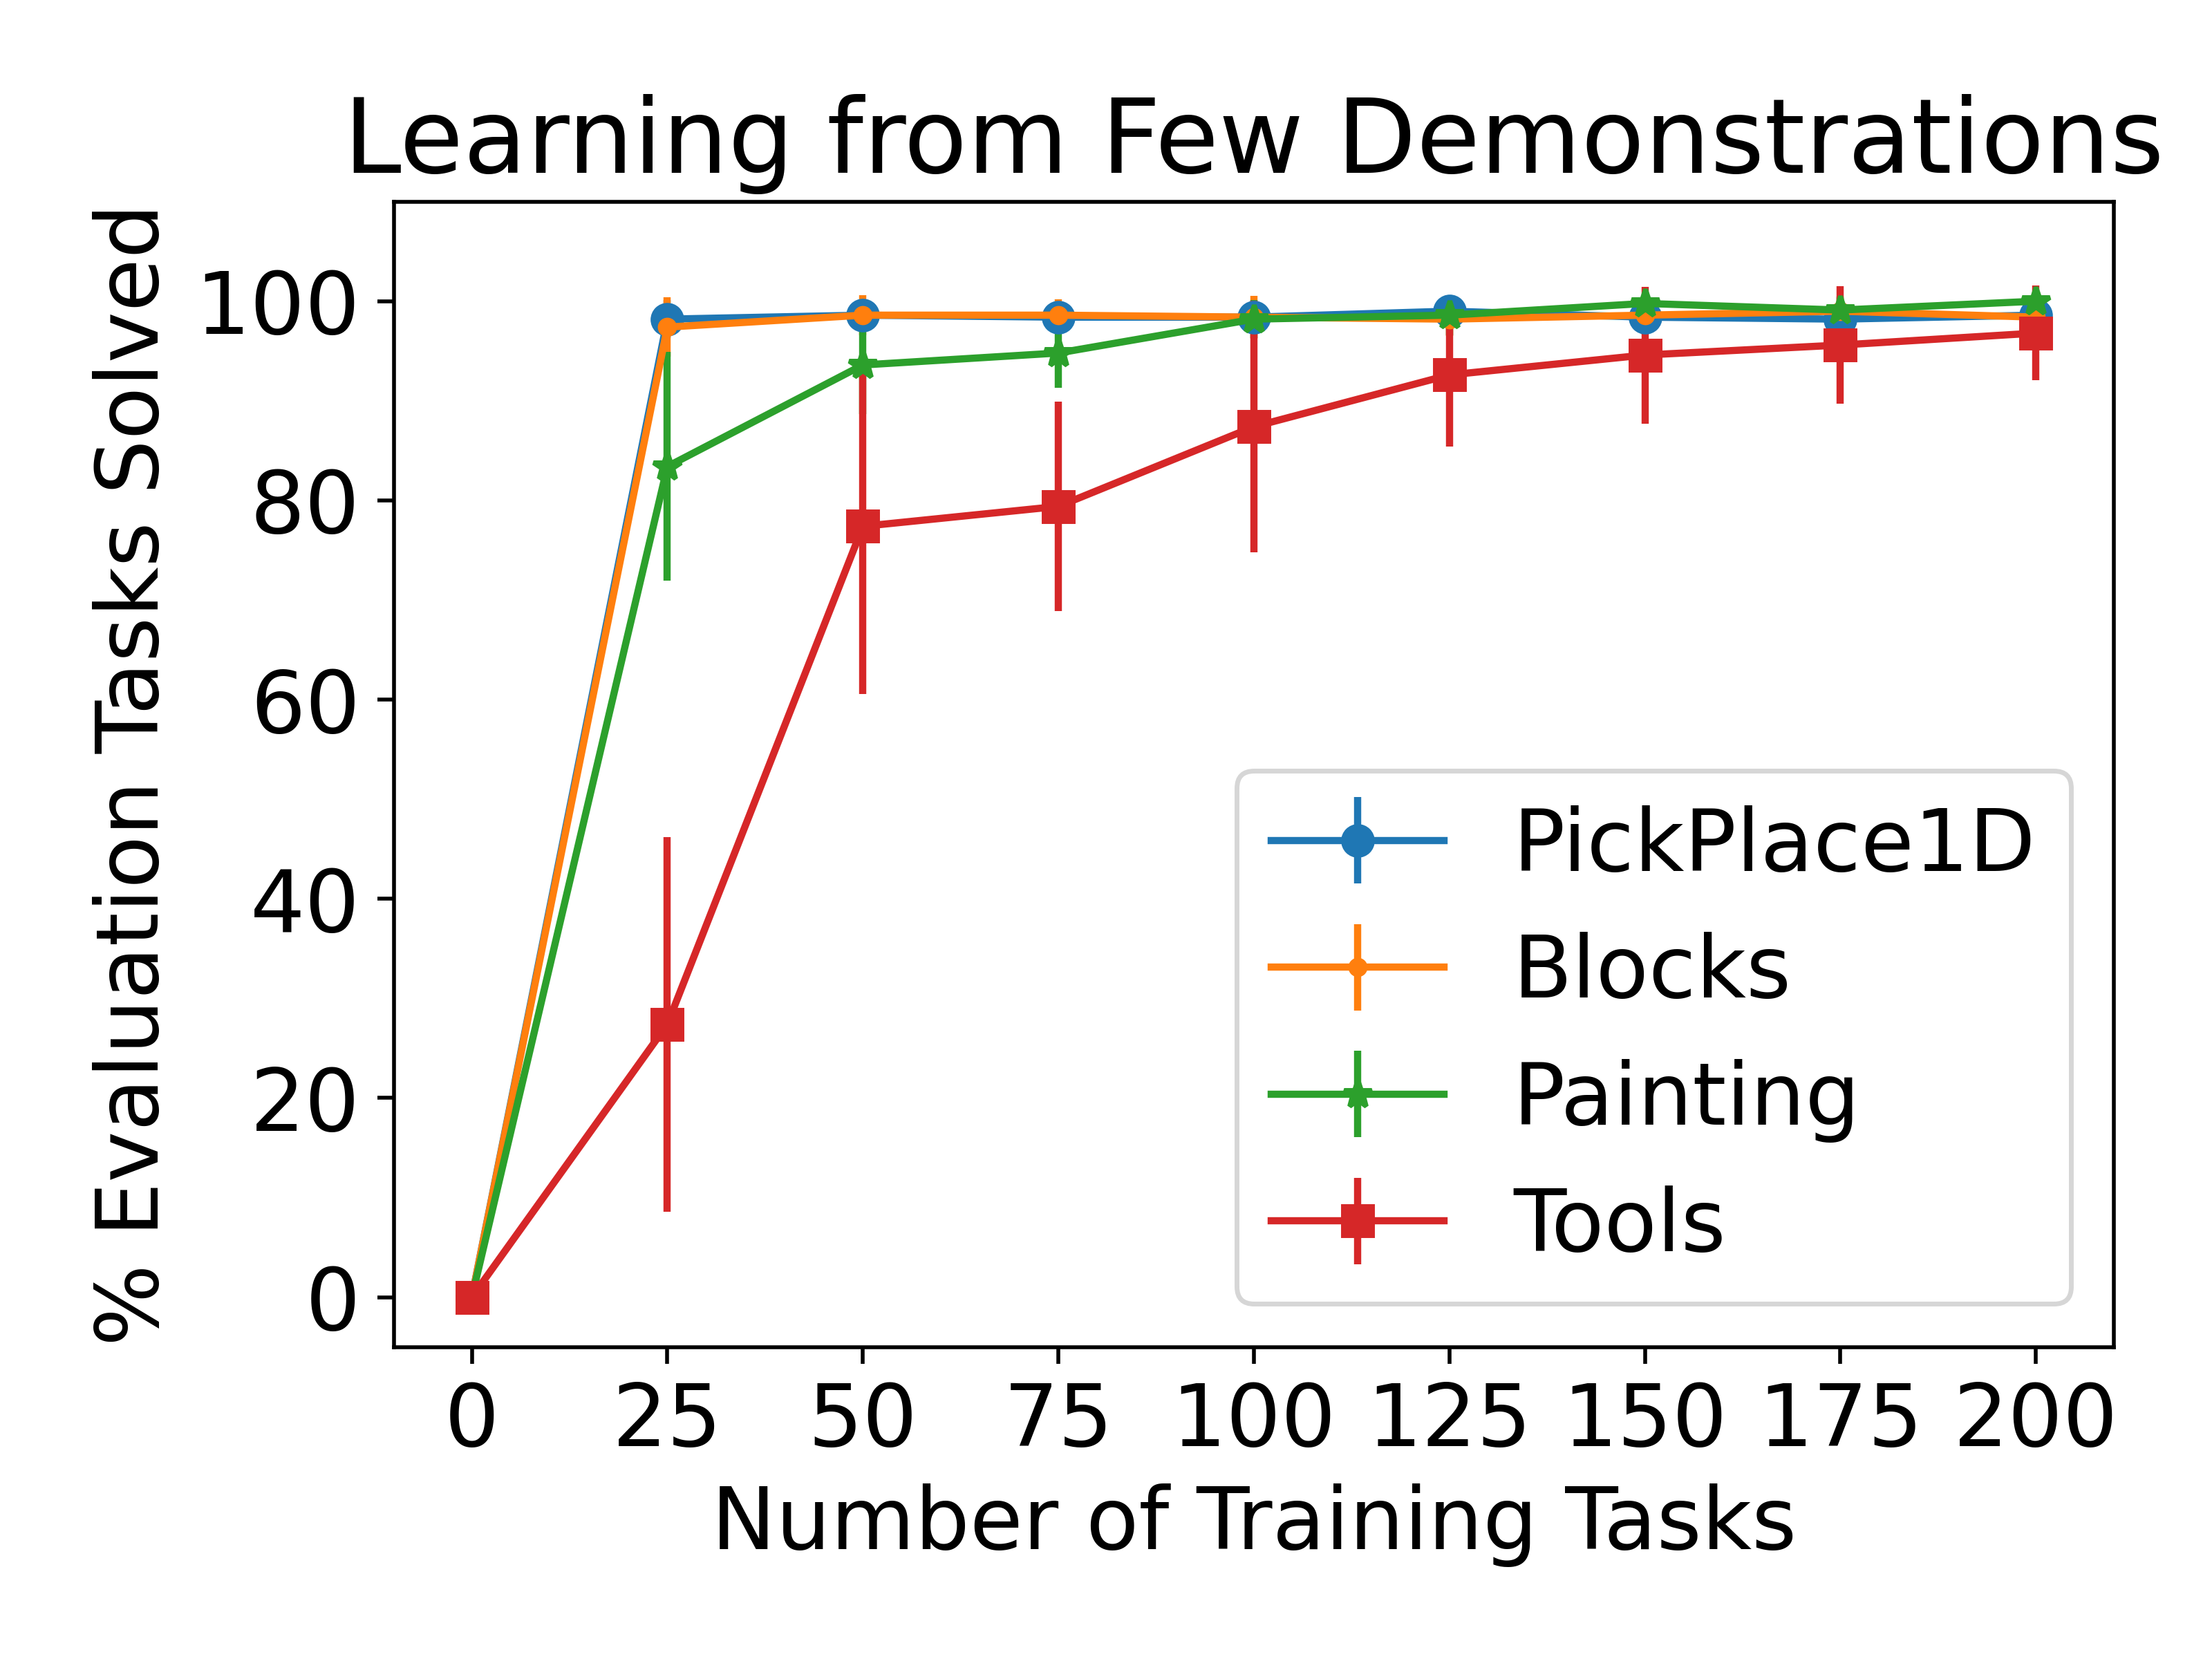
\includegraphics[width=0.29\textwidth]{figures/num_demos.png}
\end{wrapfigure}

The figure on the right illustrates the data efficiency of Ours. Each point shows a mean over 10 seeds, with standard deviations shown as vertical bars.
We often obtain very good evaluation performance within just 50 demonstrations.

In \tabref{tab:ablations}, the results for No Invent show that, as expected, the goal predicates alone are completely insufficient for most tasks.
Comparing Ours to Down Eval shows that assuming downward refinability at evaluation time works for PickPlace1D, Blocks, and Painting, but not for Tools.
We also find that the learned predicates (Ours) are on par with, and sometimes \emph{better than}, hand-designed predicates (Manual).
For instance, consider PickPlace1D, where the learned predicates are 7.5x better.
The manually designed predicates were \texttt{Held(?block)} and \texttt{HandEmpty()}, and the always-given goal predicate \texttt{Covers(?block, ?target)}.
In addition to inventing two predicates that are equivalent to \texttt{Held} and \texttt{HandEmpty}, Ours invented two more: $\texttt{P3(?block)} \triangleq \forall \texttt{?t}\ .\ \lnot \texttt{Covers(?block, ?t)}$, and $\texttt{P4(?target)} \triangleq \forall \texttt{?b}\ .\ \lnot \texttt{Covers(?b, ?target)}$. 
Intuitively, \texttt{P3} means ``the given block is not on any target,'' while \texttt{P4} means ``the given target is clear.'' 
\texttt{P3} gets used in an operator precondition for picking, which reduces the branching factor of abstract search.
This precondition is sensible because there is no use in moving a block once it is already on its target.
\texttt{P4} prevents considering non-refinable abstract plans that ``park'' objects on targets that must be covered by other objects.

In \appref{app:more-blocks-explanations}, we describe an additional experiment where we vary the AI planning heuristic used in abstract search.
We analyze a case in Blocks where variation in the invented predicates appears inconsequential upon initial inspection, but actually has substantial impact on planning efficiency.
This result underscores the benefit of using a surrogate objective for predicate invention that is sensitive to downstream planning efficiency.
